\documentclass[11pt]{article}
\usepackage[margin=1in]{geometry}
\geometry{letterpaper}
\usepackage{graphicx}
\usepackage{epstopdf}
\DeclareGraphicsRule{.tif}{png}{.png}{`convert #1 `dirname #1`/`basename #1 .tif`.png}

\usepackage{caption}
\usepackage{subcaption}

\usepackage{mathrsfs, amsmath}
\usepackage{amssymb}
\usepackage{empheq}
\newcommand*\widefbox[1]{\fbox{\hspace{2em}#1\hspace{2em}}}

\usepackage[autostyle]{csquotes}
\usepackage[section]{placeins}

%---------------------Listings Package--------------------%
\usepackage{listings}
\usepackage{color}
\definecolor{mygreen}{rgb}{0,0.6,0}
\definecolor{mygray}{rgb}{0.5,0.5,0.5}
\definecolor{mymauve}{rgb}{0.58,0,0.82}
\lstset{ %
  backgroundcolor=\color{white},   % choose the background color; you must add \usepackage{color} or \usepackage{xcolor}
  basicstyle=\footnotesize,        % the size of the fonts that are used for the code
  breakatwhitespace=flase,         % sets if automatic breaks should only happen at whitespace
  breaklines=false,                 % sets automatic line breaking
  captionpos=b,                    % sets the caption-position to bottom
  commentstyle=\color{mygreen},    % comment style
  deletekeywords={...},            % if you want to delete keywords from the given language
  escapeinside={\%*}{*)},          % if you want to add LaTeX within your code
  extendedchars=true,              % lets you use non-ASCII characters; for 8-bits encodings only, does not work with UTF-8
  frame=single,	                   % adds a frame around the code
  keepspaces=true,                 % keeps spaces in text, useful for keeping indentation of code (possibly needs columns=flexible)
  keywordstyle=\color{blue},       % keyword style
  language=Octave,                 % the language of the code
  otherkeywords={*,...},           % if you want to add more keywords to the set
  numbers=left,                    % where to put the line-numbers; possible values are (none, left, right)
  numbersep=5pt,                   % how far the line-numbers are from the code
  numberstyle=\tiny\color{mygray}, % the style that is used for the line-numbers
  rulecolor=\color{black},         % if not set, the frame-color may be changed on line-breaks within not-black text (e.g. comments (green here))
  showspaces=false,                % show spaces everywhere adding particular underscores; it overrides 'showstringspaces'
  showstringspaces=false,          % underline spaces within strings only
  showtabs=false,                  % show tabs within strings adding particular underscores
  stepnumber=2,                    % the step between two line-numbers. If it's 1, each line will be numbered
  stringstyle=\color{mymauve},     % string literal style
  tabsize=2,	                   % sets default tabsize to 2 spaces
  title=\lstname                   % show the filename of files included with \lstinputlisting; also try caption instead of title
}
%-----------------------------------------------------------------%

%-------------------Landscape Package------------------%
\usepackage{pdflscape}
%-----------------------------------------------------------------%

\title{Numerical Methods\\[0.1in] ECSE 543 - Assignment 3}
\author{Mido Assran - 260505216}
\date{\today}


\begin{document}
\maketitle

\section*{Question 1}
\vspace*{-0.1in}
\noindent\rule{\textwidth}{0.4pt}

\subsection*{Part a}
We interpolate the first six points of the BH data, denoted $x_1, x_2, \ldots, x_6$, using full-domain Lagrange Polynomials, each defined over the domain $D$, where
$$
D = [x_1, x_6]
$$
That is, we estimate the function being interpolated, $y(x)$, by six polynomials, each of degree five and defined over the entire domain $D$. The mathematical representation is
\begin{equation}
    \label{eq:lagrange_polynomial}
    y(x) = \sum^6_{j=1} a_j L_j(x), \quad x \in D
\end{equation}
where $L_j(x)$ is a fifth degree Lagrange Polynomial, and $a_j$ is a model parameter - scalar. The class \textit{LagrangeInterpolator} is used to perform the interpolation. The class is initialized with the domain points and corresponding range points - the six B and H data samples in this case. Subsequently, the initializer creates the Lagrange Polynomials corresponding to each of the six data points, and determines the associated model parameters as well.

The model parameters the set of $a_j$, are expected to simply be equal to the corresponding range points, the set of $y_j$. Nonetheless, we determine these model parameters by solving a least squares problem minimizing the error in our Lagrange Polynomial representation using a 2-norm metric relative to the target data points (the set of $\{y(x)\}$). The least squares problem is modified so that the matrix is positive definite, and then is subsequently solved using our previously created Choleski Decomposition. The implementation is provided in the listing. As expected, the result is simply that the the model parameters, the set of $a_j$, are simply equal to the corresponding range points, the set of $y_j$.

The Lagrange Polynomials are represented by the \textit{LagrangePolynomial} class contained in the \textit{polynomial\_collective.py} file. The \textit{LagrangePolynomial} class takes as input the set of domain points $\{x\}$, and the subscript index $j$. Upon initialization, the \textit{LagrangePolynomial} class creates the following polynomial:
\begin{align*}
L_j(x) &= \frac{F_j(x)}{F_j(x_j)}\\
\text{where}\\
F_j(x) &= \Pi_{r=1:6, \ r \neq j} \  (x - x_r)
\end{align*}
This polynomial is created by performing a series of binomial multiplications and a scalar division. The binomial operations are performed using the \textit{Polynomial} class represented in the \textit{polynomial.py} file. Once the $LagrangePolynomial$ is initialized, it can be evaluated by simply calling its instance method $evaluate(x)$, which takes as input a domain point at which to evaluate the Lagrange Polynomial, and returns the resulting scalar.\\
\textsc{\footnotesize *Note that the implementation works with any number of domain points, but in our mathematical representations we show only six points since those are what are used in this subsection of the assignment.}

Now back to the \textit{LagrangeInterpolator} class. After it determines its model parameters, $\{a_j\}$, and the corresponding Lagrange Polynomials, $\{L_j\}$, it can be used to interpolate the data simply by calling its $interpolate()$ instance method. This method returns a Python lambda, i.e a functional method, which evaluates equation (\ref{eq:lagrange_polynomial}). Figures \ref{fig:L_BH_first_six} and \ref{fig:L_HB_first_six} show the corresponding interpolations of B vs H and H vs B respectively. The console outputs in the Figures also showcase the closed form expanded Lagrange Polynomial for each the B vs H and the H vs B interpolations. \textbf{This result is certainly plausible, and could lie close to the true B vs H curve over this range.}

\begin{figure}[!hbp]
	\begin{center}
		\begin{minipage}{ \textwidth}
			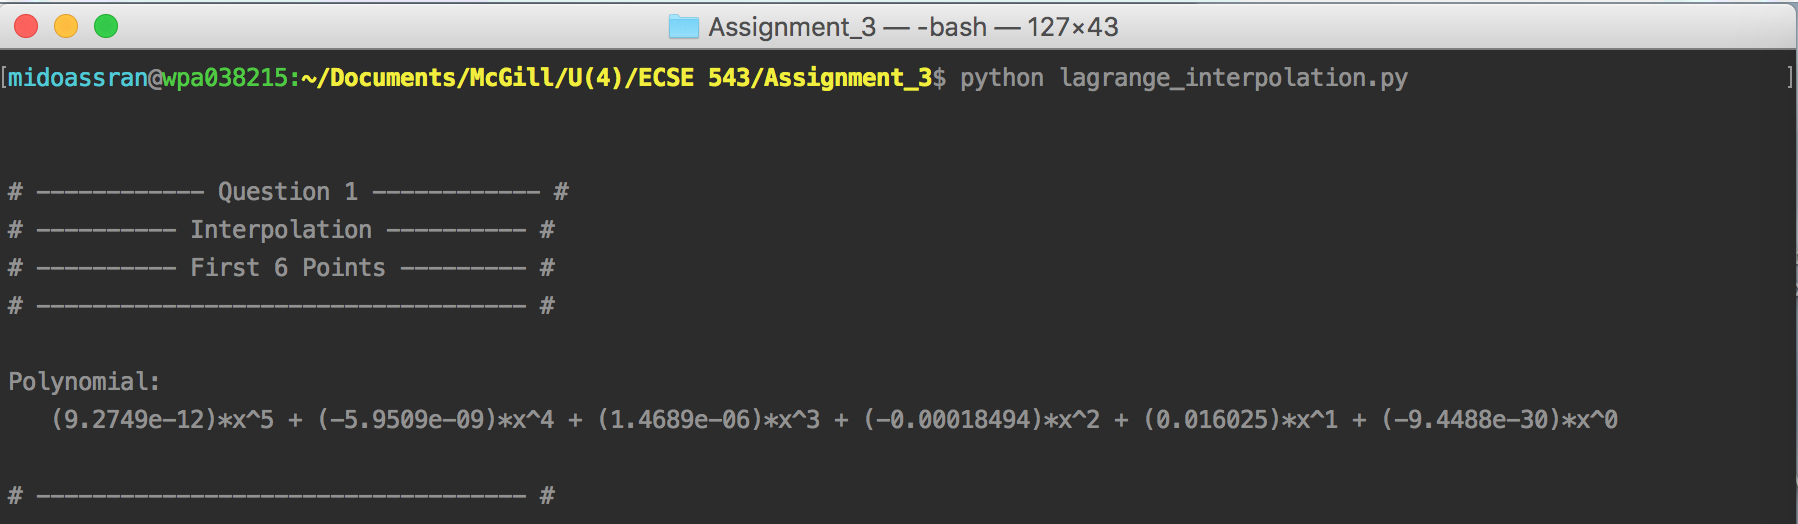
\includegraphics[width= \textwidth]{o_L_BH_first_six.png}\\
		\end{minipage}
		\begin{minipage}{ \textwidth}
			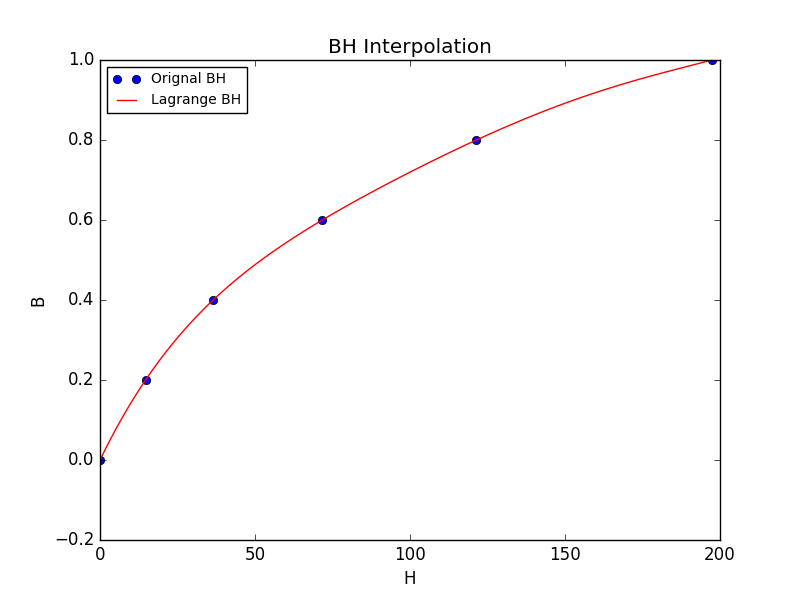
\includegraphics[width=\textwidth]{L_BH_first_six.png}\\
		\end{minipage}
		\caption{\label{fig:L_BH_first_six}B vs H interpolation using first six points}
	\end{center}
\end{figure}
\begin{figure}[!hbp]
	\begin{center}
		\begin{minipage}{ \textwidth}
			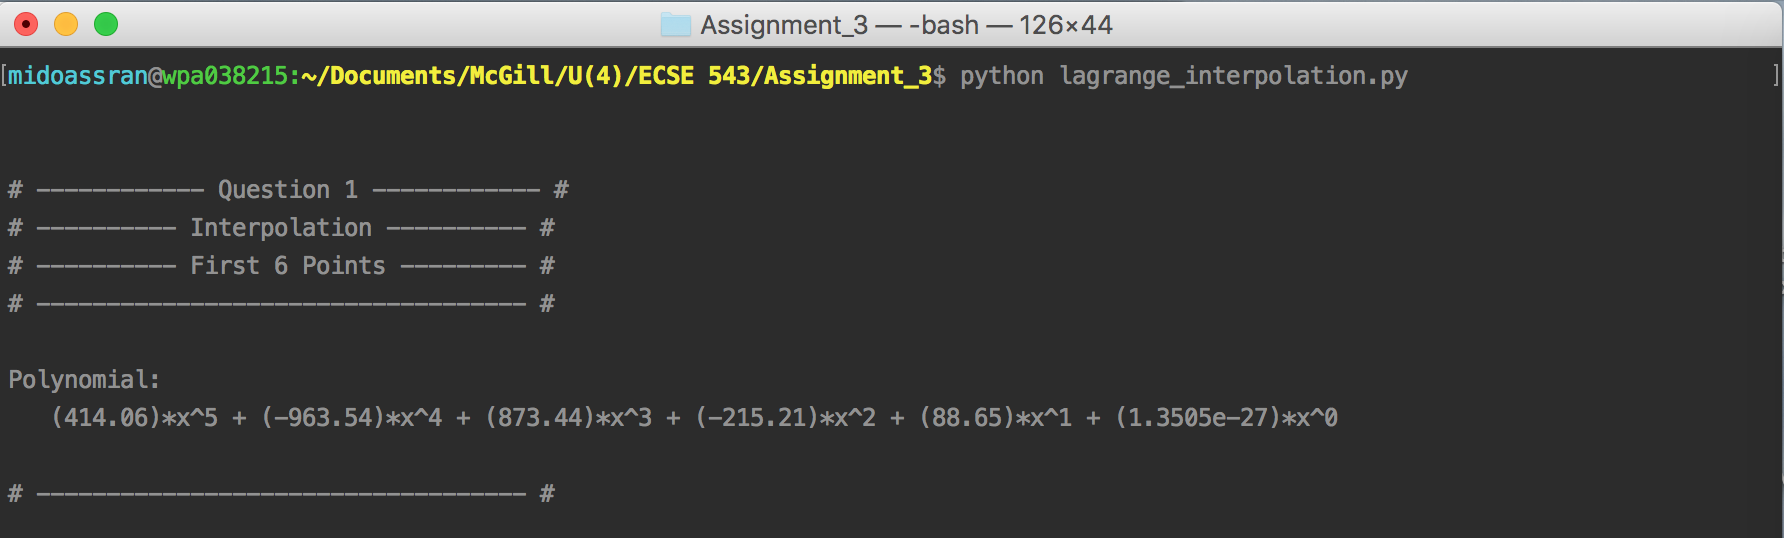
\includegraphics[width= \textwidth]{o_L_HB_first_six.png}\\
		\end{minipage}
		\begin{minipage}{ \textwidth}
			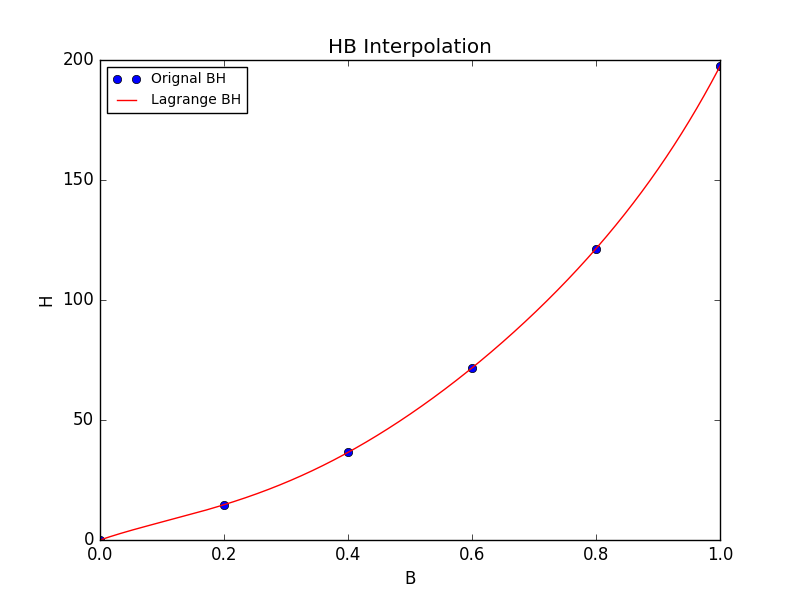
\includegraphics[width=\textwidth]{L_HB_first_six.png}\\
		\end{minipage}
		\caption{\label{fig:L_HB_first_six}H vs B interpolation using first six points}
	\end{center}
\end{figure}

\FloatBarrier
\subsection*{Part b}
Full-domain Lagrange Interpolation is once again performed: the same interpolation implementation code is used, except now the data used for the interpolation are the six points at $B = 0, 1.3, 1.4, 1.7, 1.8, 1.9$.  Figures \ref{fig:L_BH_sep_six} and \ref{fig:L_HB_sep_six} show the corresponding interpolations of B vs H and H vs B respectively. The console outputs in the figures also showcases the closed form expanded Lagrange Polynomial for each the B vs H and the H vs B interpolations. \textbf{This result is not plausible.}

\begin{figure}[!hbp]
	\begin{center}
		\begin{minipage}{ \textwidth}
			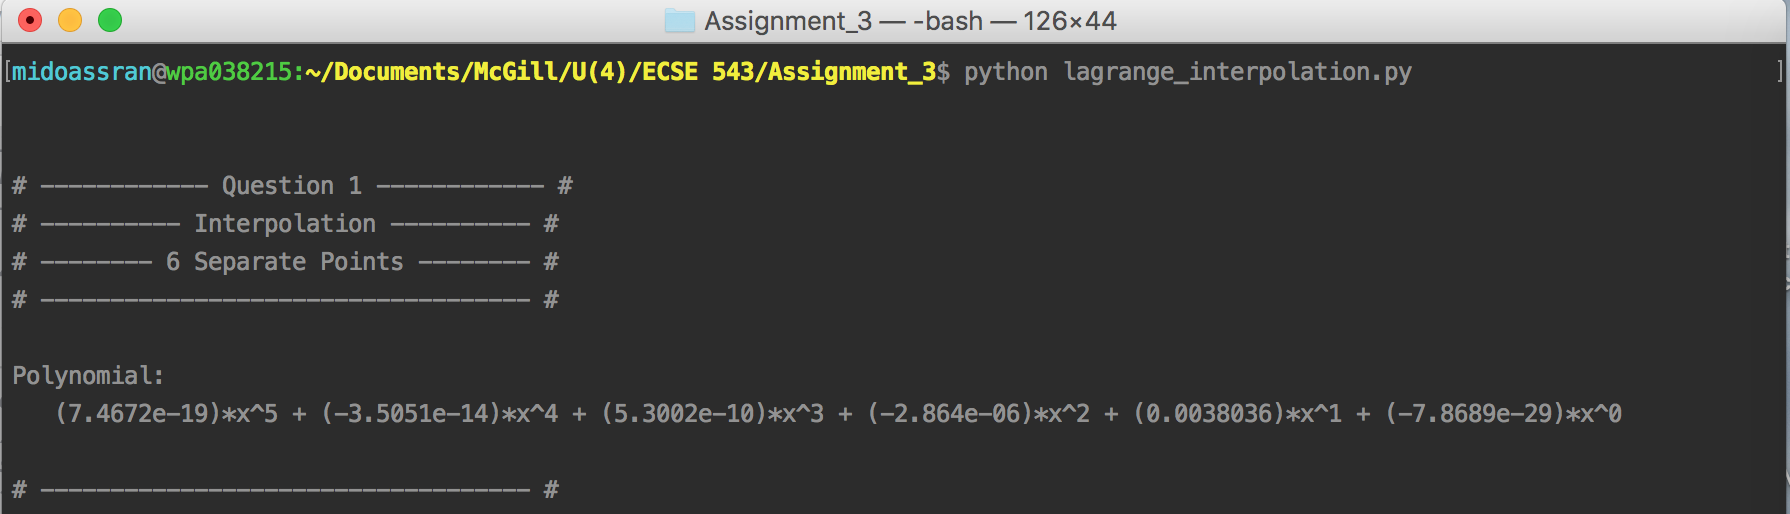
\includegraphics[width= \textwidth]{o_L_BH_sep_six.png}\\
		\end{minipage}
		\begin{minipage}{ \textwidth}
			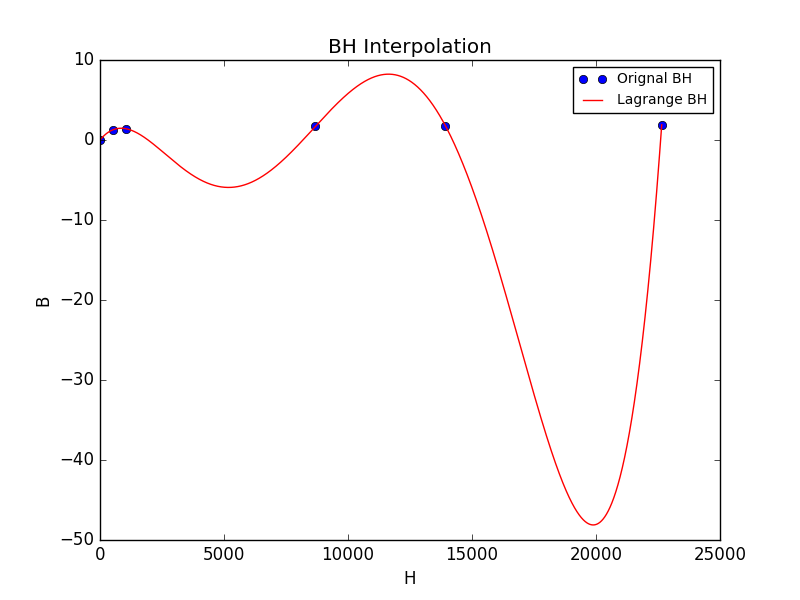
\includegraphics[width=\textwidth]{L_BH_sep_six.png}\\
		\end{minipage}
		\caption{\label{fig:L_BH_sep_six}B vs H interpolation using separate six points}
	\end{center}
\end{figure}
\begin{figure}[!hbp]
	\begin{center}
		\begin{minipage}{ \textwidth}
			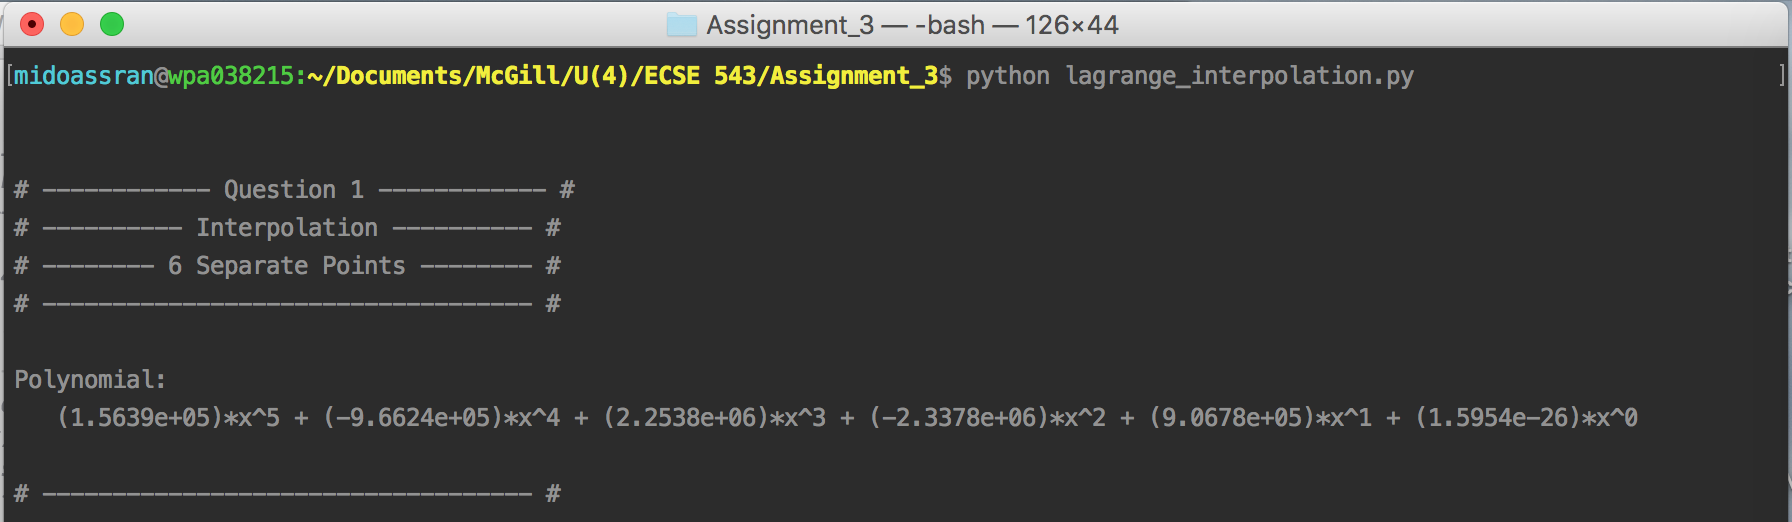
\includegraphics[width= \textwidth]{o_L_HB_sep_six.png}\\
		\end{minipage}
		\begin{minipage}{ \textwidth}
			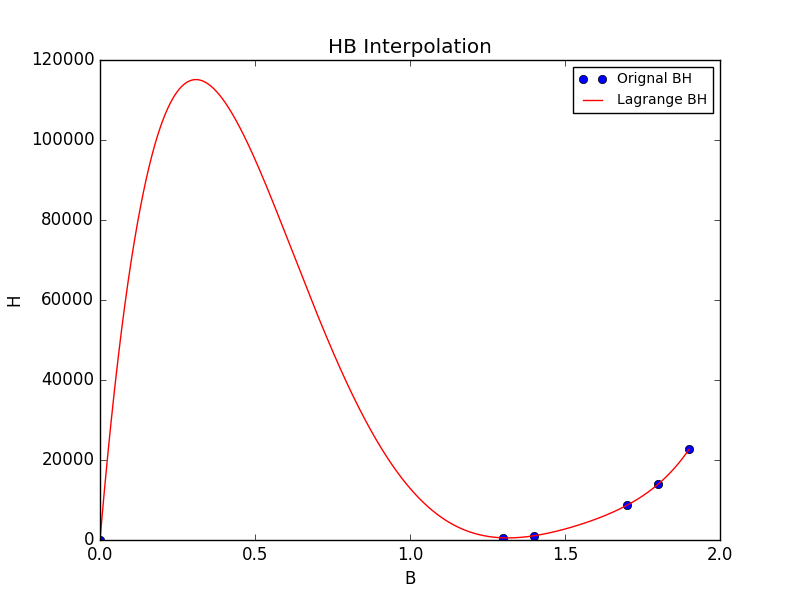
\includegraphics[width=\textwidth]{L_HB_sep_six.png}\\
		\end{minipage}
		\caption{\label{fig:L_HB_sep_six}H vs B interpolation using separate six points}
	\end{center}
\end{figure}

\FloatBarrier
\subsection*{Part c}
As was seen, full-domain Lagrange Polynomial representations are susceptible to ``wiggles'' when the domain and target points are not regularly interspersed. Hermite Polynomial representations are less susceptible to such issues since they incorporate first order information (i.e. the slopes). We take data from the six points corresponding to $B = 0, 1.3, 1.4, 1.7, 1.8, 1.9$, and construct subdomain Hermite Polynomials. We choose to use the six points to construct five non-overlapping subdomains, denoted $D_i$, where each sub-domain is made up of two points from the dataset. Therefore, we estimate the function to be interpolated, $y(x)$, by creating a two-point Hermite Polynomial representation (cubic) for each subdomain. Our function being interpolated, $y(x)$, is estimated by the piecewise representation:
\begin{align}
    y(x) =
    &\left\{\;
        \begin{array}{r@{\;}l}
            \sum^2_{j=1} a_j U_j(x) + b_j V_j(x), \quad \text{for} \quad x \in D_1\\[0.1in]
            \sum^3_{j=2} a_j U_j(x) + b_j V_j(x), \quad \text{for}\quad x \in D_2\\[0.1in]
            \sum^4_{j=3} a_j U_j(x) + b_j V_j(x), \quad \text{for}\quad x \in D_3\\[0.1in]
            \sum^5_{j=4} a_j U_j(x) + b_j V_j(x), \quad \text{for} \quad x \in D_4\\[0.1in]
            \sum^6_{j=5} a_j U_j(x) + b_j V_j(x), \quad \text{for} \quad x \in D_5 \label{eq:hermite_polynomial}
        \end{array}
    \right.
\end{align}
where
\begin{align}
    \begin{array}{r@{\;}l}
        D_1 = [x_1, x_2]\\[0.1in]
        D_2 = (x_2, x_3]\\[0.1in]
        D_3 = (x_3, x_4]\\[0.1in]
        D_4 = (x_4, x_5]\\[0.1in]
        D_5 = (x_5, x_6]\\[0.1in]
    \end{array}
\end{align}
Even though each Hermite Polynomial sum is actually defined over a closed domain, the aggregate subdomain polynomials are only defined over the semi-open interval to avoid overlap (the choice to open up the lower subinterval was completely arbitrary).

The class \textit{HermiteSubdomainInterpolator} is used to perform the interpolation. The class is initialized with the domain points and the corresponding range points - the six B and H data samples in this case. Subsequently the initializer creates two Hermite Polynomials for each of the five subdomains, and determines the associated model parameters as well.

The Hermite Polynomials are represented by the \textit{HermitePolynomial} class contained in the \textit{polynomial\_collective.py} file. The \textit{HertmiePolynomial} class has two public instance methods: \textit{evaluate\_U(x, j, dom)} and \textit{evaluate\_V(x, j, dom)} which take as input the the set of domain points over which the subdomain polynomial is to be defined (two points in this example), the subscript index $j$, and the point $x$ in the subdomain at which to evaluate the $U_j$ or $V_j$ components of the Hermite Polynomial. In a two-point subdomain, we define the polynomials over domain $D_i$ as
\begin{align*}
    U_j(x) &= [1 - 2 \cdot L^{\prime}_j(x_j) \cdot (x-x_j)]L^2_j(x), &\text{for} \quad x, x_j \in D_i\\
    V_j(x) &= (x-x_j) \cdot L^2_j(x), &\text{for} \quad x, x_j \in D_i\\
    \text{where}&\\
    L_j(x) &= \frac{x - x_k}{x_j - x_k}, &\text{for} \quad x, x_k, x_j \in D_i, \ \text{and}\ k \neq j\\
    L^{\prime}_j(x) &= \frac{1}{x_j - x_k}, &\text{for} \quad x, x_k, x_j \in D_i, \ \text{and}\ k \neq j
\end{align*}

The model parameters are the set of $a_j$ and $b_j$. The $a_j$ are chosen to be equal to the corresponding range points (the set of $y_j$), and the $b_j$ are chosen to be equal to the corresponding range derivatives $\frac{d y_j}{d x}$ - i.e the derivative of the function to be interpolated evaluated at the point $x_j$. To find the six slopes, we use a three point weighted average. Say we want to find the slope at the point $(y_j, x_j)$. Then we define the posterior and the priori slopes:
$$s_{pos} = \frac{y_{j+1} - y_j}{x_{j+1} - x_j}$$
$$s_{pri} = \frac{y_{j} - y_{j-1}}{x_{j} - x_{j-1}}$$
and take the slope at the point $(y_j, x_j)$, denoted $s_j$, to be
$$\boxed{s_j = w \cdot s_{pos} + (1 - w) \cdot s_{pri}}$$
where the weight $w$ is
$$w = \frac{s_{pri}}{s_{pos} + s_{pri}}$$
The result is that the prior and posterior slopes have an equilibrated representation in the slope estimate, without either one overpowering the other. Obviously for the first and last points in our domain we simply only use the posterior and the prior slopes respectively since there is no third point to be leveraged. If we were to simply define the slope at point $(y_j, x_j)$ to be $\frac{y_{j+1} - y_{j-1}}{x_{j+1} - x_{j-1}}$, then the much larger slope would overpower the much smaller slope, and the interpolation would overshoot. Similarly, if we only use the posterior or the prior slopes, then we would be discarding valuable information.

Now back to the \textit{HermiteSubdomainInterpolator} class. After it determines its model parameters, $\{a_j, b_j\}$, and the corresponding Hermite Polynomials, $\{U_j, V_j\}$, it can be used to interpolate the data simply by calling its \textit{interpolate()} instance method. This method returns a Python lambda, i.e. a functional method, which evaluates equation (\ref{eq:hermite_polynomial}).
\textsc{\footnotesize *Note that the implementation works with any number of domain points, but in our mathematical representations we show only six points since those are what are used in this subsection of the assignment.}

The result of the interpolation is shown in Figure \ref{fig:H_BH_sep_six}, where both the B vs H and the H vs B interpolations are shown. Clearly our weighted average works extremely well in both cases when the posterior is much larger than the prior (HB interpolation), and when the prior is much larger than the posterior (BH interpolation). \textbf{This result is certainly plausible and could lie close to the true BH curve.}

\begin{figure}[!hbp]
	\begin{center}
		\begin{minipage}{ 0.8\textwidth}
			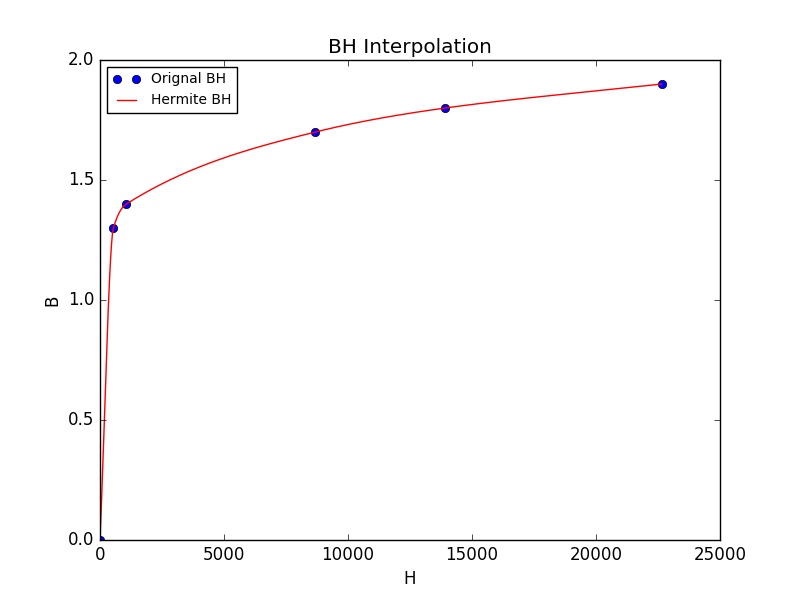
\includegraphics[width= \textwidth]{H_BH_sep_six.png}\\
		\end{minipage}
		\begin{minipage}{ 0.8\textwidth}
			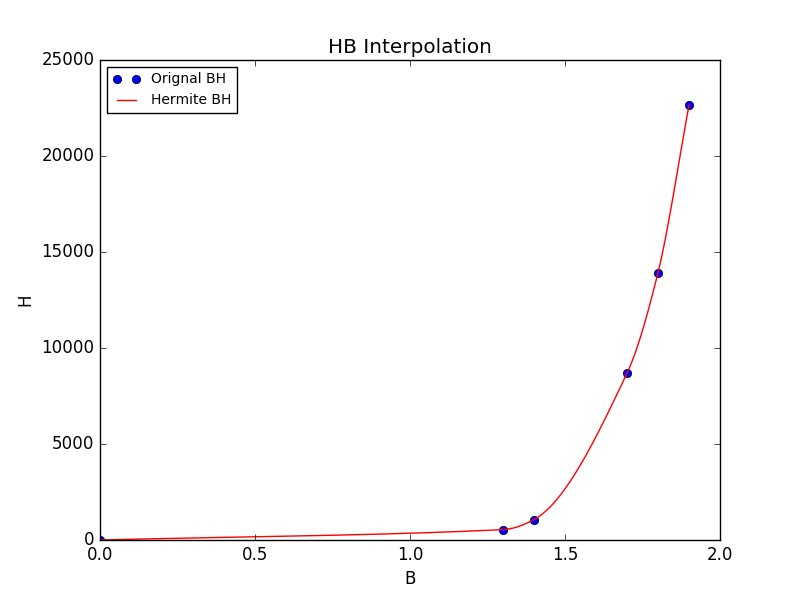
\includegraphics[width=\textwidth]{H_HB_sep_six.png}\\
		\end{minipage}
		\caption{\label{fig:H_BH_sep_six}BH interpolation using separate six points}
	\end{center}
\end{figure}

\FloatBarrier
\subsection*{Part d}
Here we derive a non-linear equation for the magnetic flux in the iron core in Figure \ref{fig:iron_core}. We construct the magnetic circuit shown in Figure \ref{fig:mag_circ}, where $R_c$ is the reluctance of the core, $R_g$ is the reluctance of the air gap, $\psi$ is the magnetic flux, and $M$ is the magnetomotive force. The constituent equation is
\begin{equation}
    \label{eq:mag_circ}
    (R_g + R_c) \cdot \psi = M
\end{equation}
where
\begin{align*}
    \begin{array}{r@{\;}l}
        M &= N \cdot I\\[0.1in]
        R_g &= \frac{L_g}{A\mu_0}\\[0.1in]
        R_c &= \frac{L_c}{A\mu}
    \end{array}
\end{align*}
$N$ is the number of turns of the coil, $I$ is the current through the coil, $A$ is the cross-sectional area of the core, $\mu_0$ is the permeability of free space, and $\mu$ is the permeability of the core, which is dependent on the magnetic flux. Therefore the reluctance of the core can be expressed as a function of the magnetic flux
$$R_c = \frac{L_c}{A \cdot \frac{B}{H(B)}}$$
or even more directly
$$R_c = \frac{L_c}{A \cdot \frac{\frac{\psi}{A}}{H(\psi)}}$$
which simplifies to
$$R_c = \frac{L_c \cdot H(\psi)}{\psi}$$
where $H(\psi)$ is the magnetic field intensity which is a function of the magnetic flux density, however since the cross-section of the core is a constant, we simply write the flux density dependence $H(B)$ as a magnetic flux dependence instead $H(\psi)$. Substituting into equation (\ref{eq:mag_circ}) and reordering we have:
$$\boxed{f(\psi) = R_g \cdot \psi + L_c \cdot H(\psi) - M = 0}$$
\begin{figure}[!hbp]
	\begin{center}
		\begin{minipage}{ 0.4\textwidth}
			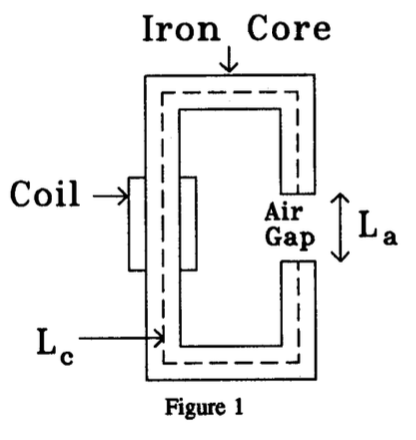
\includegraphics[width= \textwidth]{iron_core.png}\\
			\caption{\label{fig:iron_core}Iron core}
		\end{minipage}
		\quad
		\begin{minipage}{ 0.5\textwidth}
			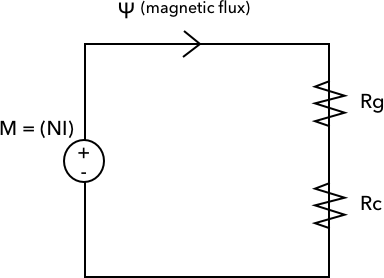
\includegraphics[width=\textwidth]{mag_circ.png}\\
    			\caption{\label{fig:mag_circ}Magnetic circuit}
		\end{minipage}
	\end{center}
\end{figure}

\FloatBarrier
\subsection*{Part e}
Here we solve the non-linear equation derived in Part d using the Newton-Raphson method. The first step is to find a piecewise-linear interpolation of the BH data to represent the $H(\psi)$ term. To construct a piecewise-linear interpolation of the data we choose to use a two-point subdomain Lagrange Polynomial interpolation, since such an interpolation defined over a subdomain would create an order one polynomial. We construct $n-1$ non-overlapping subdomains from the $n$ BH points,  denoted $D_i$, where each sub-domain is made up of two points from the dataset. Therefore, we estimate the function to be interpolated, $H(B)$, by creating a two-point Lagrange Polynomial representation (linear) for each subdomain. Our function being interpolated, $H(B)$, is estimated by the piecewise representation:
\begin{align}
    H(B) =
    \left\{\;
        \begin{array}{r@{\;}l}
            &\sum^2_{j=1} a_j L_j(B), \quad \text{for} \quad B \in D_1\\[0.1in]
            &\sum^3_{j=2} a_j L_j(B), \quad \text{for}\quad B \in D_2\\[0.1in]
            &\vdots \\[0.1in]
            &\sum^n_{j=n-1} a_j L_j(B), \quad \text{for} \quad B \in D_{n-1} \label{eq:subdomain_lagrange_polynomail}
        \end{array}
    \right.
\end{align}
where
\begin{align}
    \begin{array}{r@{\;}l}
        D_1 &= [B_1, B_2]\\[0.1in]
        D_2 &= (B_2, B_3]\\[0.1in]
	\vdots \\[0.1in]
        D_{n-1} &= (B_{n-1}, B_{n}]\\[0.1in]
    \end{array}
\end{align}

The class \textit{LagrangeSubdomainInterpolator} is used to perform the interpolation. The class is initialized with the domain points and the corresponding range points - the $n$ B and H data samples in this case. Subsequently the initializer creates two Lagrange Polynomials for each of the $n-1$ subdomains, and determines the associated model parameters as well.

The Lagrange Polynomials are represented by the \textit{LagrangePolynomial} class contained in the \textit{polynomial\_collective.py} file. The \textit{LagrangePolynomial} class takes as input the set of domain points $\{B\}$, and the subscript index $j$. Upon initialization, the \textit{LagrangePolynomial} class creates the following polynomial:
\begin{align*}
L_j(B) &= \frac{F_j(B)}{F_j(B_j)}\\
\text{where}\\
F_j(B) &= (B - B_r), &\text{for} \quad B, B_j \in D_i, \ \text{and}\ r \neq j
\end{align*}
This polynomial is created by performing a series of binomial multiplications and a scalar division. The binomial operations are performed using the \textit{Polynomial} class represented in the \textit{polynomial.py} file. Once the $LagrangePolynomial$ is initialized, it can be evaluated by simply calling its instance method $evaluate(B)$, which takes as input a domain point at which to evaluate the Lagrange Polynomial, and returns the resulting scalar. The model parameters, the set of $a_j$, are simply chosen to be equal to the corresponding range points, the set of $B_j$.

Now the next step is to solve equation (\ref{eq:mag_circ}) using the $H(B)$ representation interpolated in equation (\ref{eq:subdomain_lagrange_polynomail}). The \textit{NewtonRaphsonSolver} class is used to solve the non-linear equation. The solution can be obtained by calling the class' \textit{solve(starting\_guess, f, g, stopping\_ratio)} method, which takes as input the starting guess of the optimal argument, the non-linear function in the form of a Python lambda, denoted $f$, the derivative of the non-linear function in the form of a Python lambda, denoted $g$, and the ratio of the non-linear function at the final and starting argument values used as a stopping condition for the iterative solver. The Newton Raphson iterations are obtained by solving the equation
$$g^{(k)} (\psi^{(k+1)} - \psi^{(k)}) + f^{(k)} = 0$$
which gives the $\psi^{(k+1)}$ update
$$\boxed{\psi^{(k+1)} = \psi^{(k)} - \frac{f^{(k)}}{g^{(k)}}}$$
where $\psi^{(k)}$ is the estimate of the flux at the $k^{th}$ optimization iteration, $g^{(k)}$ is the derivative evaluated at $\psi^{(k)}$, and $f^{(k)}$ is the non-linear equation evaluated at $\psi^{(k)}$.

The console output is provided in Figure \ref{fig:NR_Q1}, which shows the piecewise linear representation of $H(B)$ using the Subdomain Lagrange Polynomials, and the number of steps and the final estimate of the flux highlighted in red. \textbf{It takes 3 iteration steps from a starting guess of $\psi=0$, and the final flux is $\psi=0.000161269369397$.}
\begin{figure}[!hbp]
	\begin{center}
		\begin{minipage}{ \textwidth}
			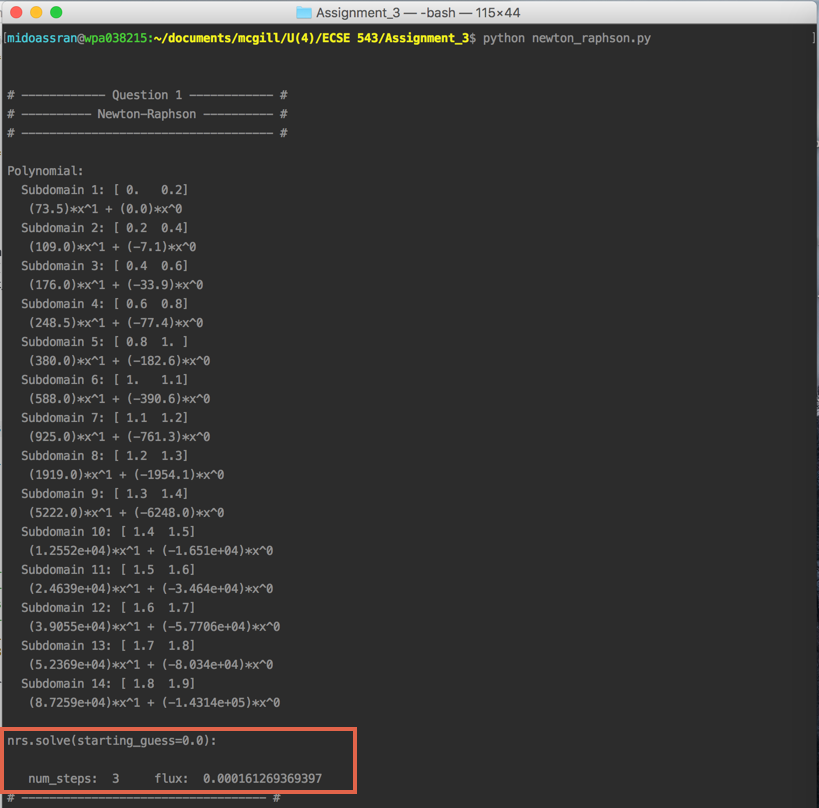
\includegraphics[width= \textwidth]{NR_Q1}\\
			\caption{\label{fig:NR_Q1}Console output of Newton Raphson solver for Part e. The piecewise linear representation of $H(B)$ using the Subdomain Lagrange Polynomials is shown. The number of steps and the final estimate of the flux are also recorded.}
		\end{minipage}
	\end{center}
\end{figure}

\FloatBarrier
\subsection*{Part f}
Here we solve the non-linear equation derived in Part d using the Successive Substitution method. We use the same implementation code as that used for the \textit{Newton Raphson} method, except in that we constantly use a derivative of $1$, rather than a variable metric. The Successive Substitution update is
$$\boxed{\psi^{(k+1)} = \psi^{(k)} - f^{(k)}}$$
The non-linear equation to be solved for
$$f(\psi) = R_g \cdot \psi + L_c \cdot H(\psi) - M = 0$$
does not converge. To get around this issue we modify non-linear equation to the form
$$\boxed{f(\psi) = (R_g \cdot \psi + L_c \cdot H(\psi) - M ) \cdot 10^{-10} = 0}$$
This form of the non-linear equation does indeed converge using the Successive Substitution method. The reasoning for scaling down the function is to flatten it out. Since we are always using a constant slope of one in each update, the lower we hit the function on the range, the shorter the distance we will travel along the $\psi$ axis. It is key that we ensure that the value of $\psi$ remain in the domain over which our piecewise linear interpolation of $H(\psi)$ is valid, otherwise we could diverge. 

The console output is provided in Figure \ref{fig:SS_Q1}, which shows the piecewise linear representation of $H(B)$ using the Subdomain Lagrange Polynomials, and the number of steps and the final estimate of the flux highlighted in red. \textbf{It takes 1172 iteration steps from a starting guess of $\psi=0$, and the final flux is $\psi=0.000161269318761$.}
\begin{figure}[!hbp]
	\begin{center}
		\begin{minipage}{ \textwidth}
			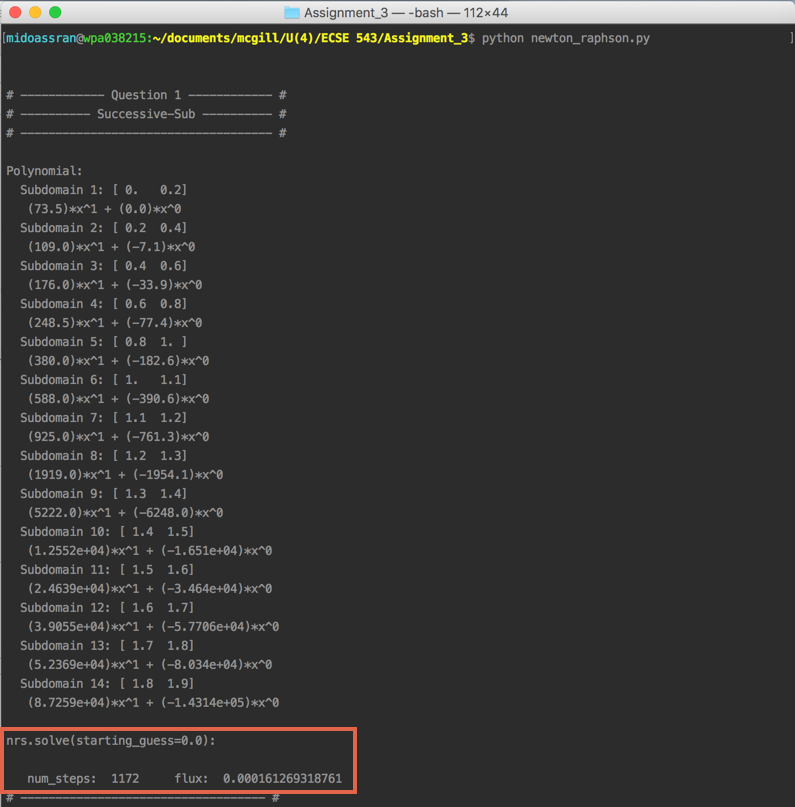
\includegraphics[width= \textwidth]{SS_Q1.png}\\
			\caption{\label{fig:SS_Q1}Console output of Successive Substitution solver for Part f. The piecewise linear representation of $H(B)$ using the Subdomain Lagrange Polynomials is shown. The number of steps and the final estimate of the flux are also recorded.}
		\end{minipage}
	\end{center}
\end{figure}

\section*{Question 2}
\vspace*{-0.1in}
\noindent\rule{\textwidth}{0.4pt}

\subsection*{Part a}
Here we derive nonlinear equations for a vector of nodal voltages, $v_n$, in the form $f(v_n)$ = 0 for the electric circuit shown in Figure \ref{fig:circuit_Q2}. The first equation, $f_1(v_1, v_2)$ is derived by carrying out a Kirchhoff Voltage Loop
$$\boxed{f_1(v_1, v_2) = v_1 - E + R \cdot I_{SA}(e^{\frac{v_1 - v_2}{kT/q}} - 1) = 0}$$
where $v_1$ and $v_2$ are the nodal voltages, $E$ is the source voltage, $R$ is the resistor's resistance, the term $I_{SA}(e^{\frac{v_1 - v_2}{kT/q}} - 1)$ is the current through diode A, $kT/q \approx 25mV$ and $I_{SA}$ is diode A's saturation current. The second equation, $f_2(v_1, v_2)$ is derived using a nodal analysis at node $v_2$
$$\boxed{f_2(v_1, v_2) = I_{SA}(e^{\frac{v_1 - v_2}{kT/q}} - 1) - I_{SB}(e^{\frac{v_2 - 0}{kT/q}} - 1) = 0}$$
where $v_1$ and $v_2$ are the nodal voltages, $E$ is the source voltage, $R$ is the resistor's resistance, the term $I_{SA}(e^{\frac{v_1 - v_2}{kT/q}} - 1)$ is the current through diode A,  the term $I_{SB}(e^{\frac{v_2}{kT/q}} - 1)$ is the current through diode B, $kT/q \approx 25mV$, $I_{SB}$ is diode B's saturation current and  $I_{SA}$ is diode A's saturation current. In vector form we have
$$\mathbf{f(\mathbf{v})} = [f_1(\mathbf{v}), f_2(\mathbf{v})]^T = 0$$
where
$$\mathbf{v} = [v_1, v_2]^T$$
\begin{figure}[!hbp]
	\begin{center}
		\begin{minipage}{0.4 \textwidth}
			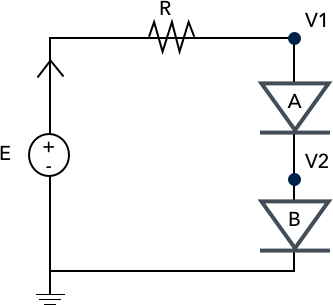
\includegraphics[width= \textwidth]{circuit_Q2.png}\\
			\caption{\label{fig:circuit_Q2}}
		\end{minipage}
	\end{center}
\end{figure}

\FloatBarrier
\subsection*{Part b}
The \textit{NewtonRaphsonSolver} class is used to solve the non-linear equation $\mathbf{f} = \mathbf{0}$. The solution can be obtained by calling the class' \textit{solve\_2D(starting\_guess, f, J, stopping\_ratio)} method, which takes as input the 2-D array input of starting guesses (the starting node voltages), the non-linear 2D function ($[f_1, f_2]$) in the form of a list of Python lambdas, the Jacobian of the non-linear functions $\mathbf{f}$, denoted by $J$, in the form of a $2 \times 2$ matrix of Python lambdas, and the minimum error used as the stopping condition for the iterative solver. The Newton Raphson iterations are obtained by solving the equation
$$\mathbf{J^{(k)}} \cdot (\mathbf{v}^{(k+1)} - \mathbf{v}^{(k)}) + \mathbf{f^{(k)}} = 0$$
which gives the $\mathbf{v^{(k+1)}}$ update
$$\boxed{\mathbf{v}^{(k+1)} = \mathbf{v}^{(k)} - (\mathbf{J^{(k)}})^{-1} \cdot \mathbf{f^{(k)}}}$$
where $\mathbf{v}^{(k)}$ is the estimate of the node voltages at the $k^{th}$ optimization iteration, $\mathbf{J}^{(k)}$ is the Jacobian evaluated at $\mathbf{v}^{(k)}$, and $\mathbf{f}^{(k)}$ is the vector of non-linear equation evaluated at $\mathbf{v}^{(k)}$. In actuality, our implementation determines $temp = - (\mathbf{J^{(k)}})^{-1} \cdot \mathbf{f^{(k)}}$ by solving 
$$(\mathbf{J^{(k)}})^T \cdot (\mathbf{J^{(k)}}) \cdot temp = - (\mathbf{J^{(k)}})^T \mathbf{f^{(k)}}$$
using our previously created Choleski Decomposition implementation. The error metric, denoted $e^{(k)}$, is simply chosen to be
$$e^{(k)} = \frac{||\mathbf{f^{(k)}}||_2}{E}$$
where we have normalized the norm of the vector of functions by the voltage-source voltage.

The console output is provided in Figure \ref{fig:o_NR_Q2}, and showcases the vector values of the voltage $\mathbf{v}^{(k)}$, the function $\mathbf{f}^{(k)}$, and the error $e^{(k)}$ at each iteration $k$. Figure \ref{fig:NR_Q2} plots the error metric on a logarithmic y axis, and fits it to an ideal quadratic convergence curve. The convergence behaviour observed is known as superlinear, or equivalently, quadratic. The mathematical representation of a quadratically convergent series is
$$\frac{1}{2^{2^{i \cdot \kappa}}}$$
where $\kappa$ is an arbitrary constant. This ideal curve is shown by the dotted blue line in Figure \ref{fig:NR_Q2}, and clearly fits the observed error's convergence curve quite well. \textbf{The convergence is quadratic.}
\begin{figure}[!hbp]
	\begin{center}
		\begin{minipage}{ \textwidth}
			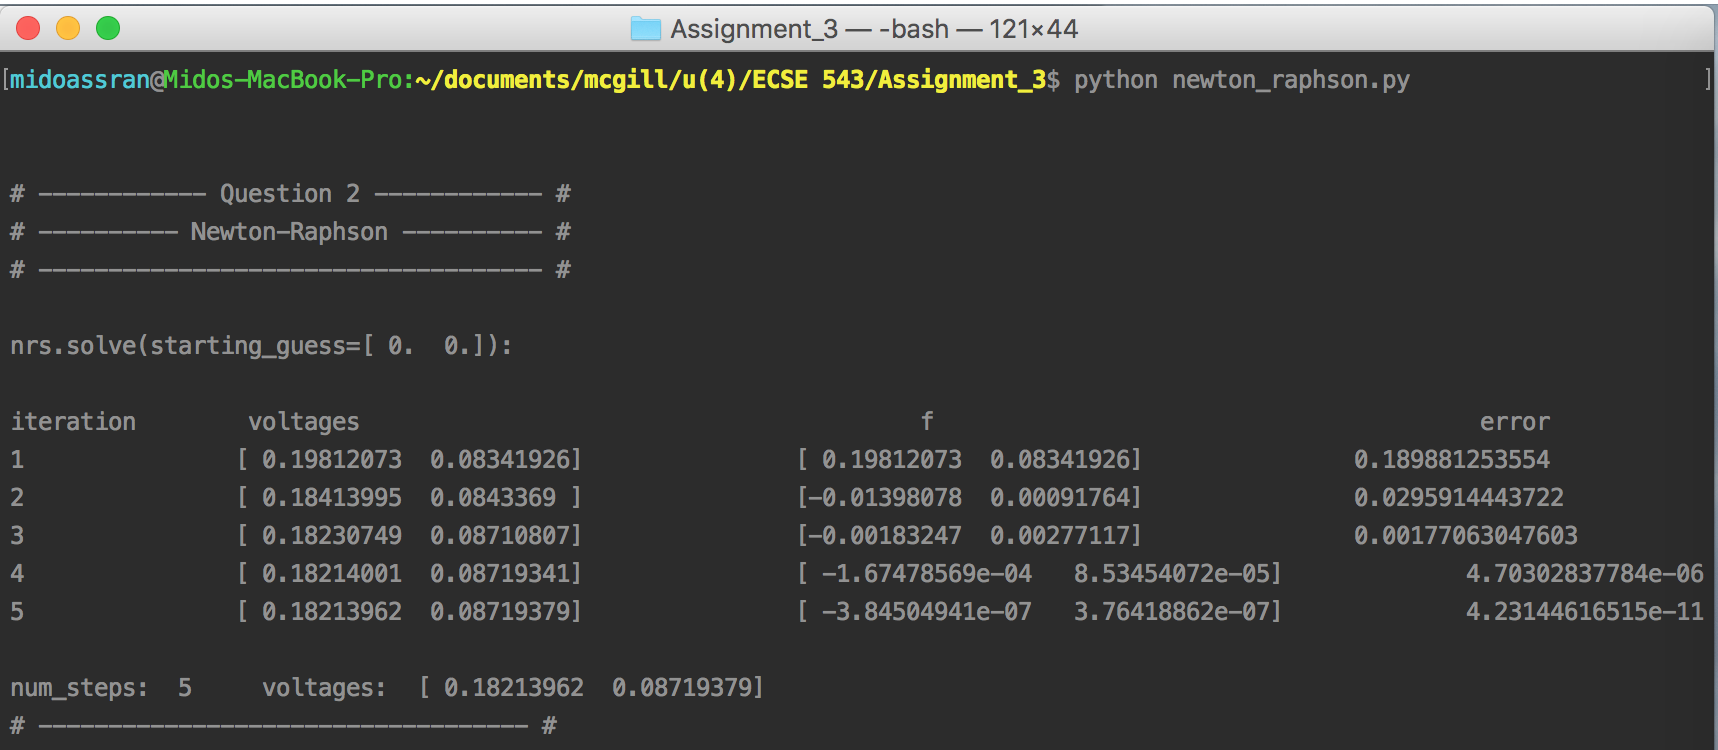
\includegraphics[width= \textwidth]{o_NR_Q2.png}\\
			\caption{\label{fig:o_NR_Q2}Console output of Newton Raphson showing the voltage estimates, the function f, and the error at each iteration.}
		\end{minipage}
		\begin{minipage}{ \textwidth}
			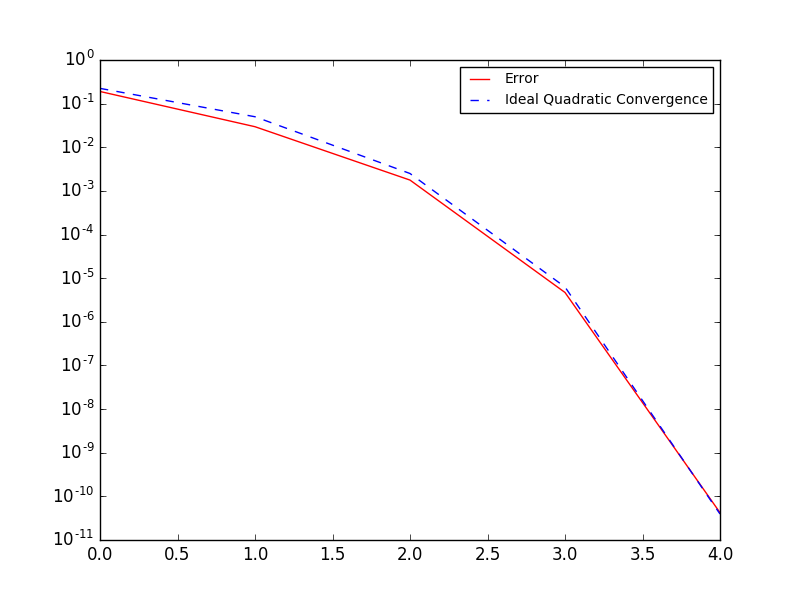
\includegraphics[width=\textwidth]{NR_Q2}\\
			\caption{\label{fig:NR_Q2}The Newton Raphson error metric plotted on a logarithmic y axis, and fitted to an ideal quadratic convergence curve.}
		\end{minipage}
	\end{center}
\end{figure}

\FloatBarrier
\section*{Question 3}
\vspace*{-0.1in}
\noindent\rule{\textwidth}{0.4pt}

\subsection*{Program implementation}
We write a program that integrates a function $f(x)$ on the interval $[x_0, x_N]$ by dividing it into subintervals and performing one-point Gauss-Legendre integration for each subinterval  a Riemann Sum fashion. The basic Gauss Legendre approximation is
$$\int^{1}_{\zeta=-1} f(\zeta) d\zeta = \sum^{n}_{i=0}w_i f(\zeta_i)$$
where we have $n+1$ unknown weights, and $n+1$ abscissa points, therefore we have $2n+2$ degrees of freedom. Therefore, the following functions, $\zeta^0, \zeta^1, \ldots, \zeta^{2n-1}$ are integrated exactly. For one point Gauss Legendre we have only one abscissa point, $\zeta_0$, and one weight, $w_0$, to be determined; consequently we have two degrees of freedom with one point Gauss Legendre, and we must solve a linear system of two equations:
\begin{align*}
    &\int^{1}_{\zeta=-1} d\zeta = w_0\\[0.1in]
    &\int^{1}_{\zeta=-1} \zeta d\zeta = w_0 \zeta_0
\end{align*}
However in general we do not wish to use the Gauss Legendre interval $[-1, 1]$, we would like to generalize this to a an arbitrary interval $[a, b]$ and solve
$$\int^{b}_{x=a} f(x) dx = \sum^{n}_{i=0}w_i f(x_i)$$
To do this we simply carry out a coordinate mapping. The result of the mapping is the new system of equations to be solved
\begin{empheq}[box=\widefbox]{align}
    &\frac{b-a}{2} \int^{1}_{\zeta=-1} d\zeta = w_0\\[0.1in]
    &\frac{b-a}{2} \int^{1}_{\zeta=-1} (\frac{b-a}{2} \zeta + \frac{b+a}{2}) d\zeta = w_0 \zeta_0
\end{empheq}
which when solved give us
\begin{empheq}[box=\widefbox]{align*}
	w_0 &= b - a\\
	\zeta_0 &= \frac{1}{2}(b+a)
\end{empheq}
where $w_0$ is the weight in the one point Gauss Legendre subinterval, and $\zeta_0$ is the abscissa in the one point Gauss Legendre subinterval. We have that the weight is equal to the interval width, and the abscissa is the midpoint of the subinterval. As a side note, this result is a common Riemann Sum technique. The error in the integral approximation is determined from the dominant term in the Taylor Series expansion of the function to be integrated, $f(x)$. For one point Gauss Legendre, the constant and linear terms will be integrated exactly, but the quadratic and higher degree terms will not. Therefore, the dominant error in one point Gauss Legendre is the quadratic term in the Taylor Series expansion. The error is simply obtained by finding the difference between the ``true'' solution and the program output.

The integration is carried out using the \textit{OnePointGaussLegendre} class, by calling its \textit{integrate(function, interval, num\_segments)} function which takes as input the function to be integrated in the form of a Python lambda, the interval over which to perform the integration, and the number of segments the interval is to be split up into. This method then performs the aforementioned logic, and returns the result of the integration (scalar).

\subsection*{Part a}
We use the program to integrate the function $f(x) = sin(x)$ on the interval $[0, 1]$ for $N$ number of segments $1, 2, \ldots , 20$. Figure \ref{fig:GL_sin} shows the base 10 logarithm of the error in the integration plotted versus the base 10 logarithm of the number of subintervals used. The console output providing the exact integration and error estimates for each number of subintervals is also shown in Figure \ref{fig:GL_sin}. The error minimization curve observed is known as a ``sublinearly convergent'' error in the literature, and corresponds to minimization of the mathematical form
$$ error \propto \frac{1}{N + 1} $$
Intuitively what this means is that when the number of segments used is quite small, it is very beneficial to increase the number of segments used. This also means that further incremental increases in the number of segments used results in less incremental benefits. That is, our error will improve very quickly initially, and then the improvements will slow down as we increase the number of segments used.

\begin{figure}[!hbp]
	\begin{center}
		\begin{minipage}{ 0.7\textwidth}
			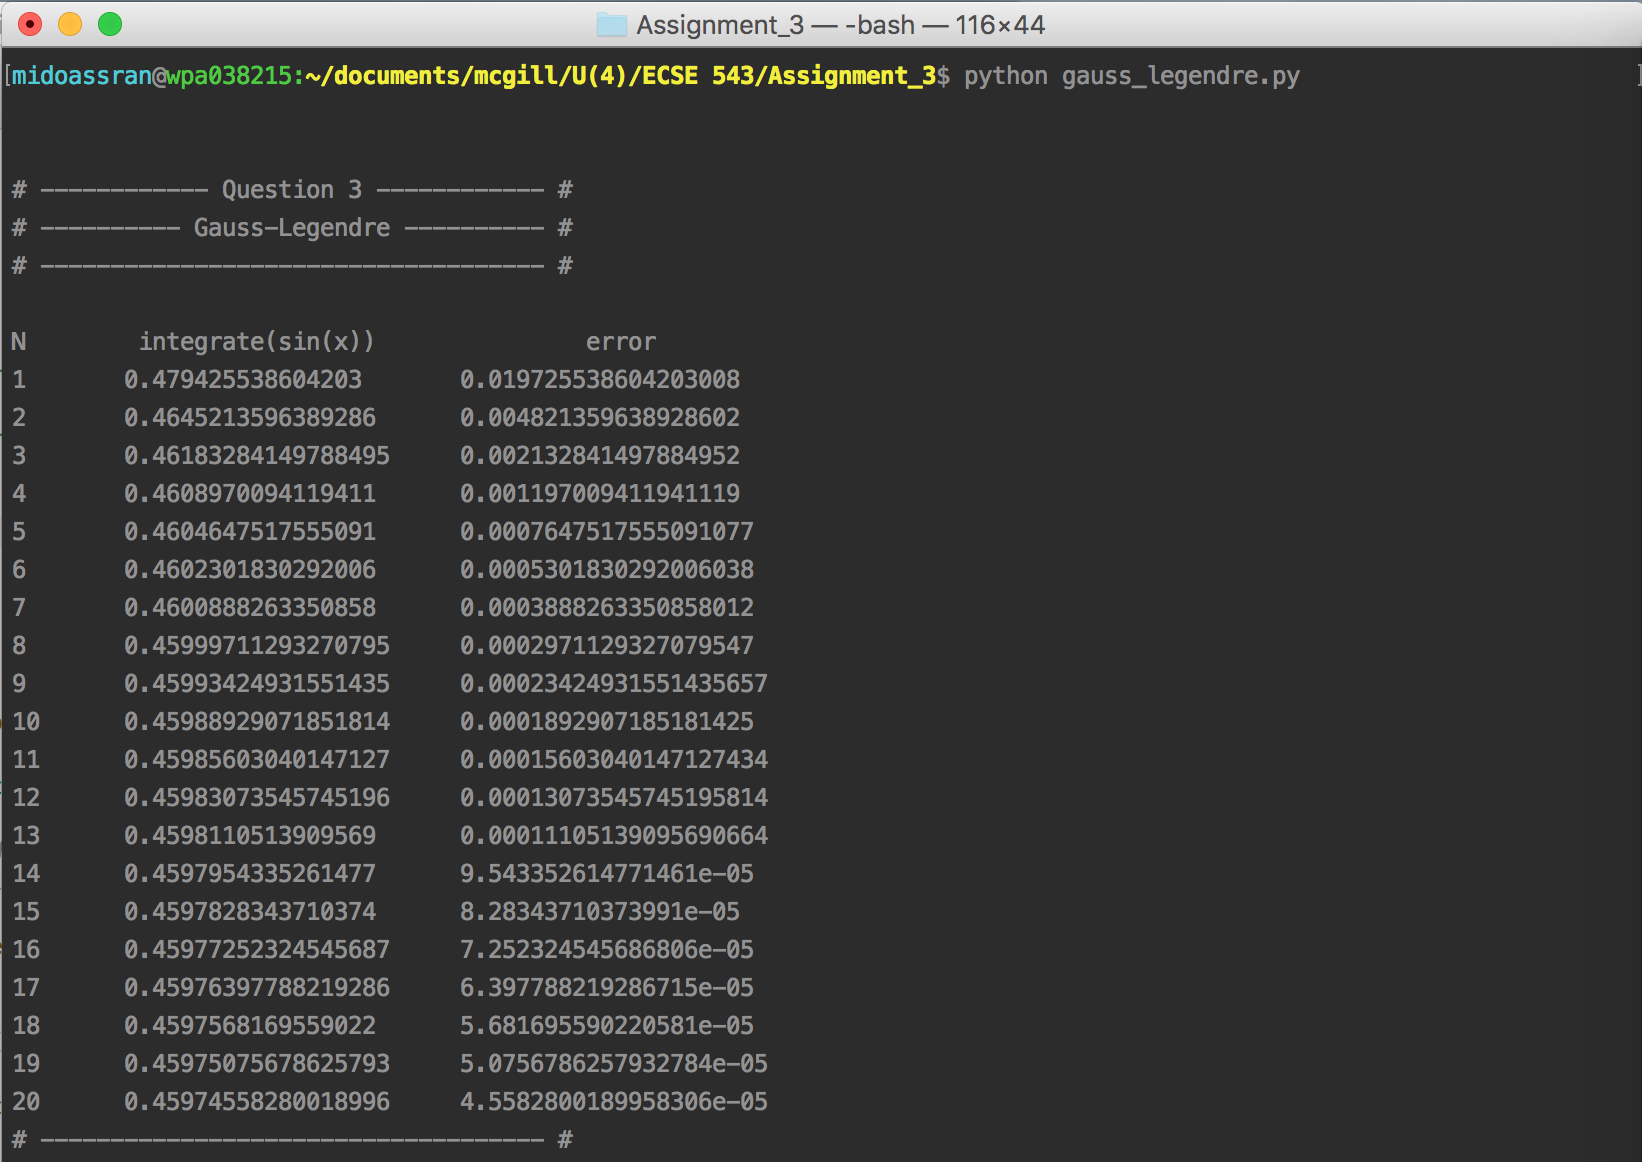
\includegraphics[width= \textwidth]{o_GL_sin.png}\\
		\end{minipage}
		\begin{minipage}{ \textwidth}
			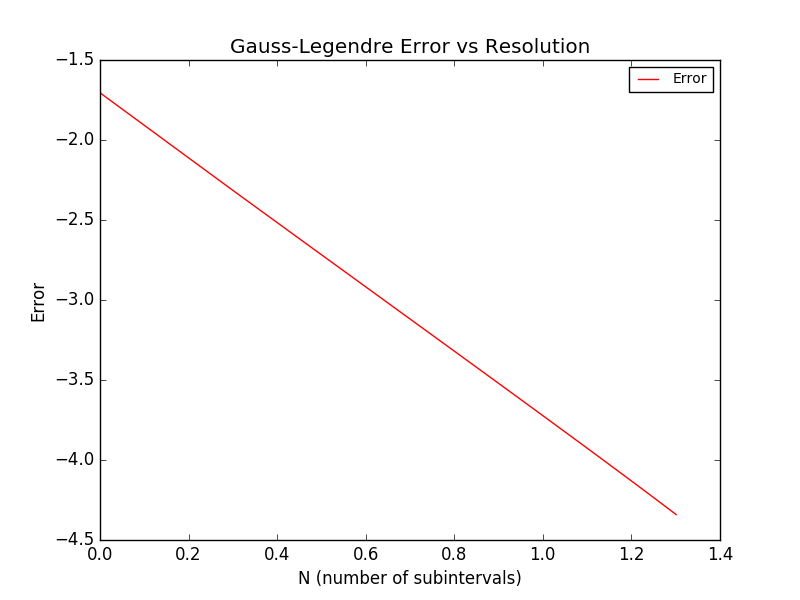
\includegraphics[width=\textwidth]{GL_sin.png}\\
		\end{minipage}
		\caption{\label{fig:GL_sin}The base 10 logarithm in the error in the Gauss Legendre integration of $sin(x)$ over the interval $[0,1]$ plotted vs the base 10 logarithm of the number of subintervals the range is broken into.}
	\end{center}
\end{figure}

\FloatBarrier
\subsection*{Part b}
We use the program to integrate the function $f(x) = ln(x)$ on the interval $[0, 1]$ for $N$ number of segments $1, 2, \ldots , 20$. Figure \ref{fig:GL_log} shows the base 10 logarithm of the error in the integration plotted versus the base 10 logarithm of the number of subintervals used. The console output providing the exact integration and error estimates for each number of subintervals is also shown in Figure \ref{fig:GL_log}. The error minimization curve observed is known as a ``sublinearly convergent'' error in the literature, and corresponds to minimization of the mathematical form
$$ error \propto \frac{1}{N + 1} $$
Intuitively what this means is that when the number of segments used is quite small, it is very beneficial to increase the number of segments used. This also means that further incremental increases in the number of segments used results in less incremental benefits. That is, our error will improve very quickly initially, and then the improvements will slow down as we increase the number of segments used. This result is very similar to that of Part a.

\begin{figure}[!hbp]
	\begin{center}
		\begin{minipage}{ 0.7\textwidth}
			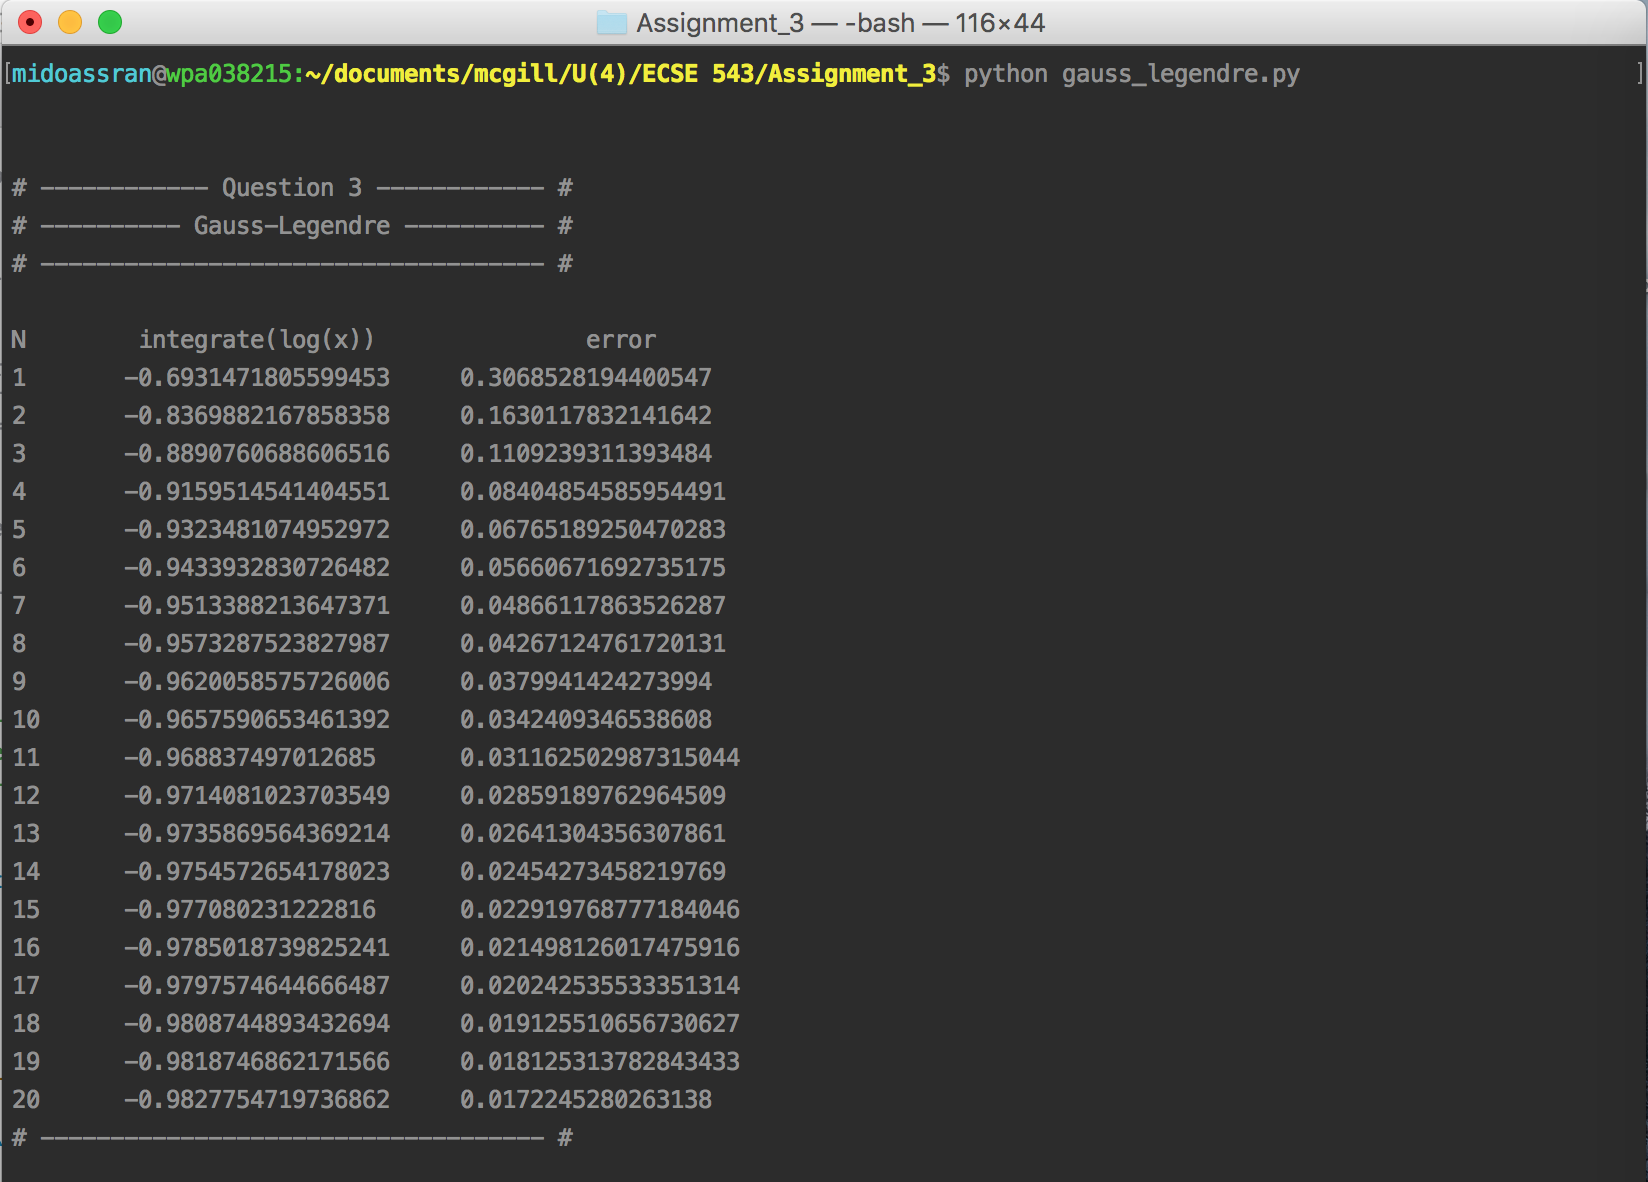
\includegraphics[width= \textwidth]{o_GL_log}\\
		\end{minipage}
		\begin{minipage}{ \textwidth}
			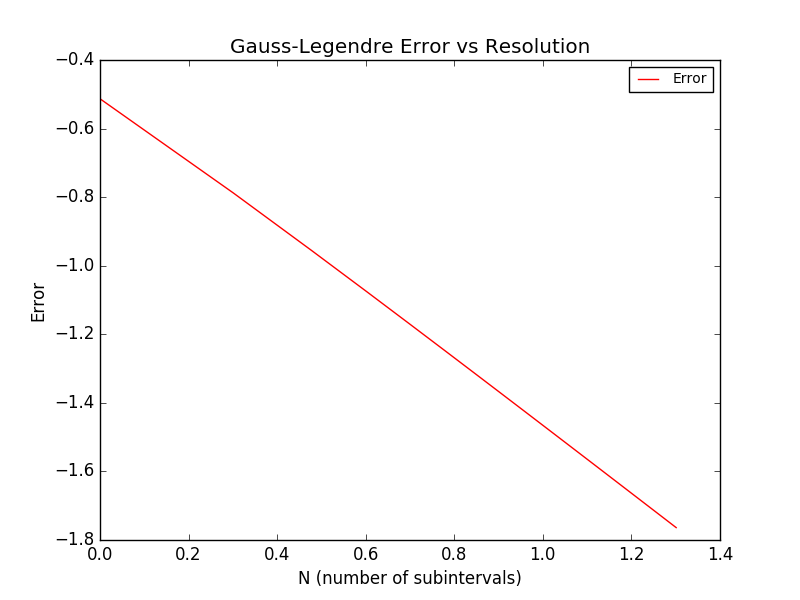
\includegraphics[width=\textwidth]{GL_log}\\
		\end{minipage}
		\caption{\label{fig:GL_log}The base 10 logarithm in the error in the Gauss Legendre integration of $ln(x)$ over the interval $[0,1]$ plotted vs the base 10 logarithm of the number of subintervals the range is broken into.}
	\end{center}
\end{figure}

\FloatBarrier
\subsection*{Part c}
We use the program to integrate the function $f(x) = ln(0.2 |sin(x)|)$ on the interval $[0, 1]$ for $N$ number of segments $1, 2, \ldots , 20$. Figure \ref{fig:GL_log_sin} shows the base 10 logarithm of the error in the integration plotted versus the base 10 logarithm of the number of subintervals used. The console output providing the exact integration and error estimates for each number of subintervals is also shown in Figure \ref{fig:GL_log_sin}. Once again, the error minimization curve observed appears to be ``sublinearly convergent'', and corresponds to minimization of the mathematical form
$$ error \propto \frac{1}{N + 1} $$
However it also appears to minimize the error faster than Part a and Part b, i.e less sublinear than Part a and Part b, but this is very difficult to judge qualitatively.

\begin{figure}[!hbp]
	\begin{center}
		\begin{minipage}{ 0.7\textwidth}
			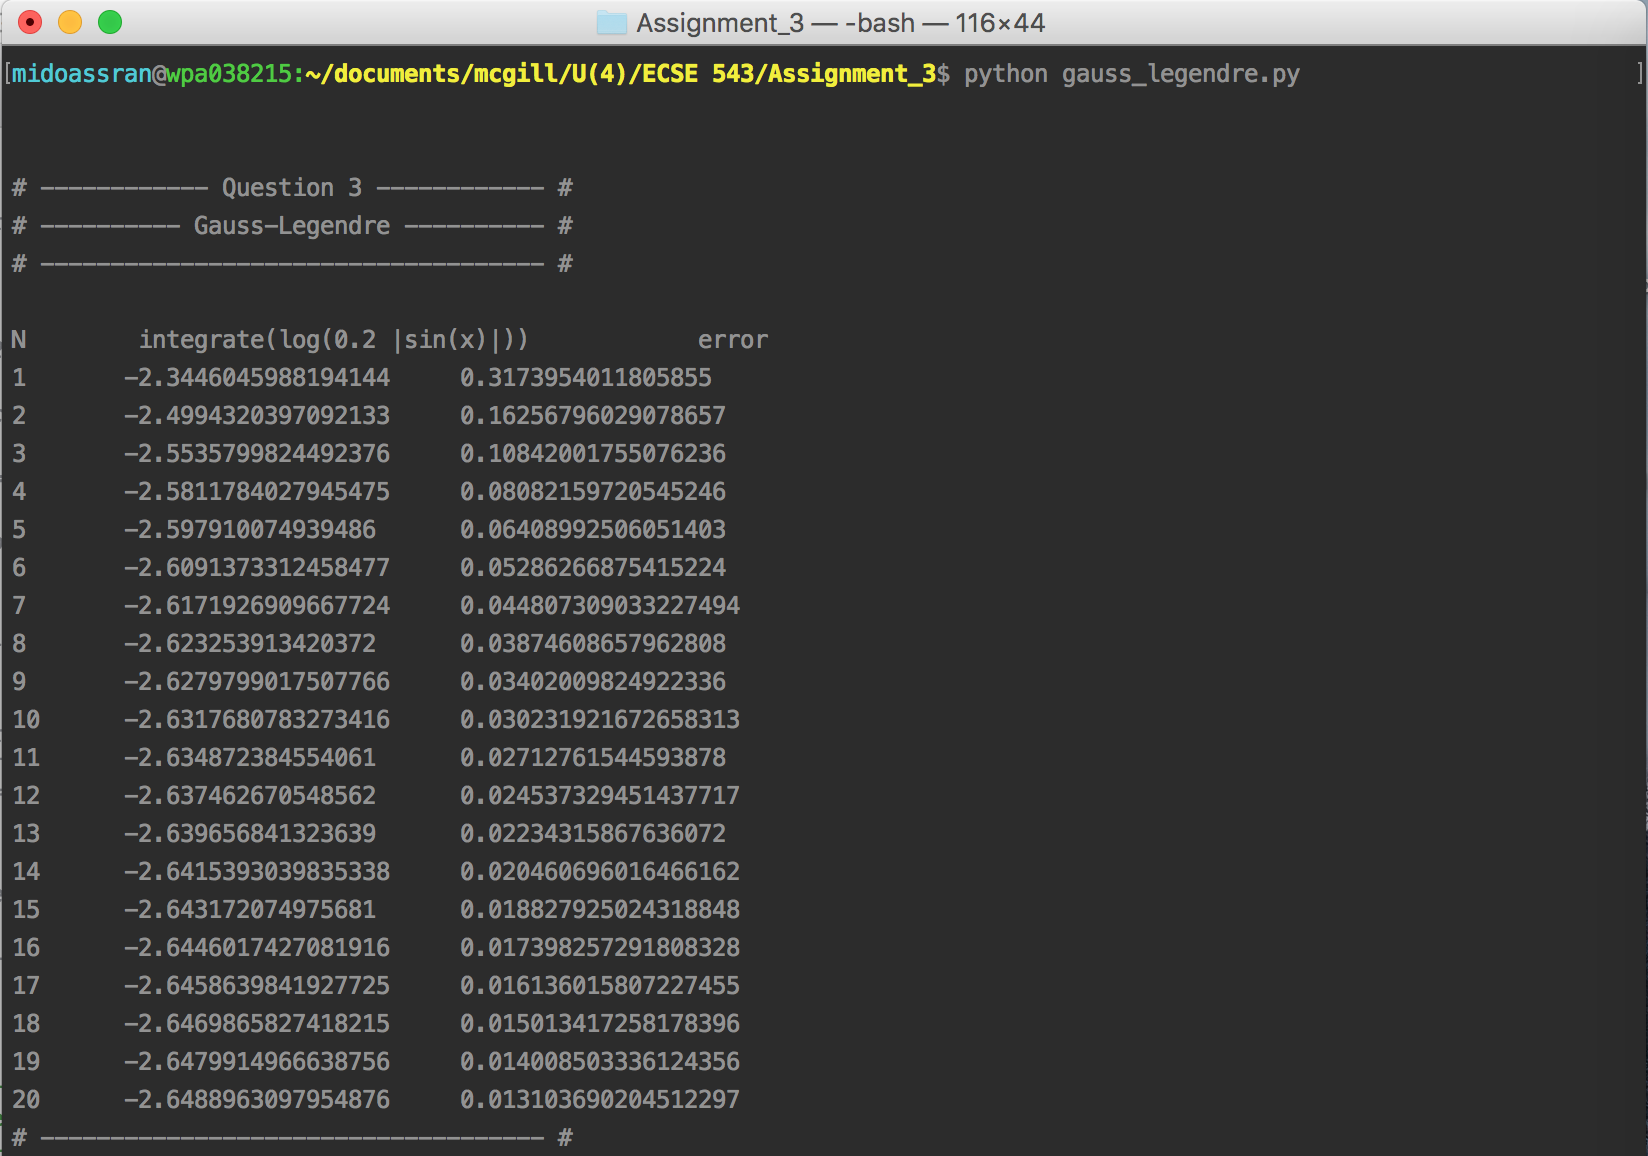
\includegraphics[width= \textwidth]{o_GL_log_sin.png}\\
		\end{minipage}
		\begin{minipage}{ \textwidth}
			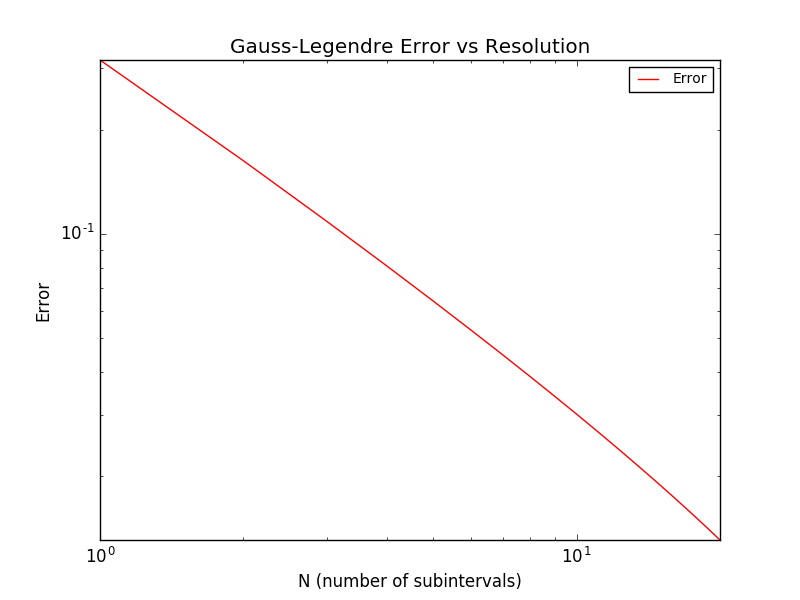
\includegraphics[width=\textwidth]{GL_log_sin}\\
		\end{minipage}
		\caption{\label{fig:GL_log_sin}The base 10 logarithm in the error in the Gauss Legendre integration of $ln(0.2 |sin(x)|)$ over the interval $[0,1]$ plotted vs the base 10 logarithm of the number of subintervals the range is broken into.}
	\end{center}
\end{figure}

\FloatBarrier
\subsection*{Part d}
Here we integrate $f(x)$ in Part b and Part c using ten unequally spaced segments. We choose to make the segment widths much smaller closer to $x = 0$, and make the segment widths larger closer to $x=1$. The integration is carried out using the \textit{OnePointGaussLegendre} class, by calling its \textit{integrate\_unequal(function, interval, num\_segments)} function which takes as input the function to be integrated in the form of a Python lambda, the interval over which to perform the integration, and the number of segments the interval is to be split up into. This method then performs the aforementioned logic, and returns the result of the integration (scalar). The result is shown in Figure \ref{fig:GL_uneven}, which shows the error in the Gauss Legendre integration of $ln(x)$ and $ln(0.2 |sin(x)|)$ over the interval $[0,1]$ for evenly spaced subintervals and unevenly spaced subintervals. \textbf{The error is lower when unevenly spaced subintervals are used. For $ln(x)$ the evenly spaced error is $0.0342409346538608$, whereas this error is $0.01600749333620799$ for unevenly spaced subintervals. For $ln(0.2 |sin(x)|)$ the evenly spaced error is $0.030231921672658313$, whereas the error is $0.012602967838622803$ for unevenly spaced subintervals.}

\begin{figure}[!hbp]
	\begin{center}
		\begin{minipage}{\textwidth}
			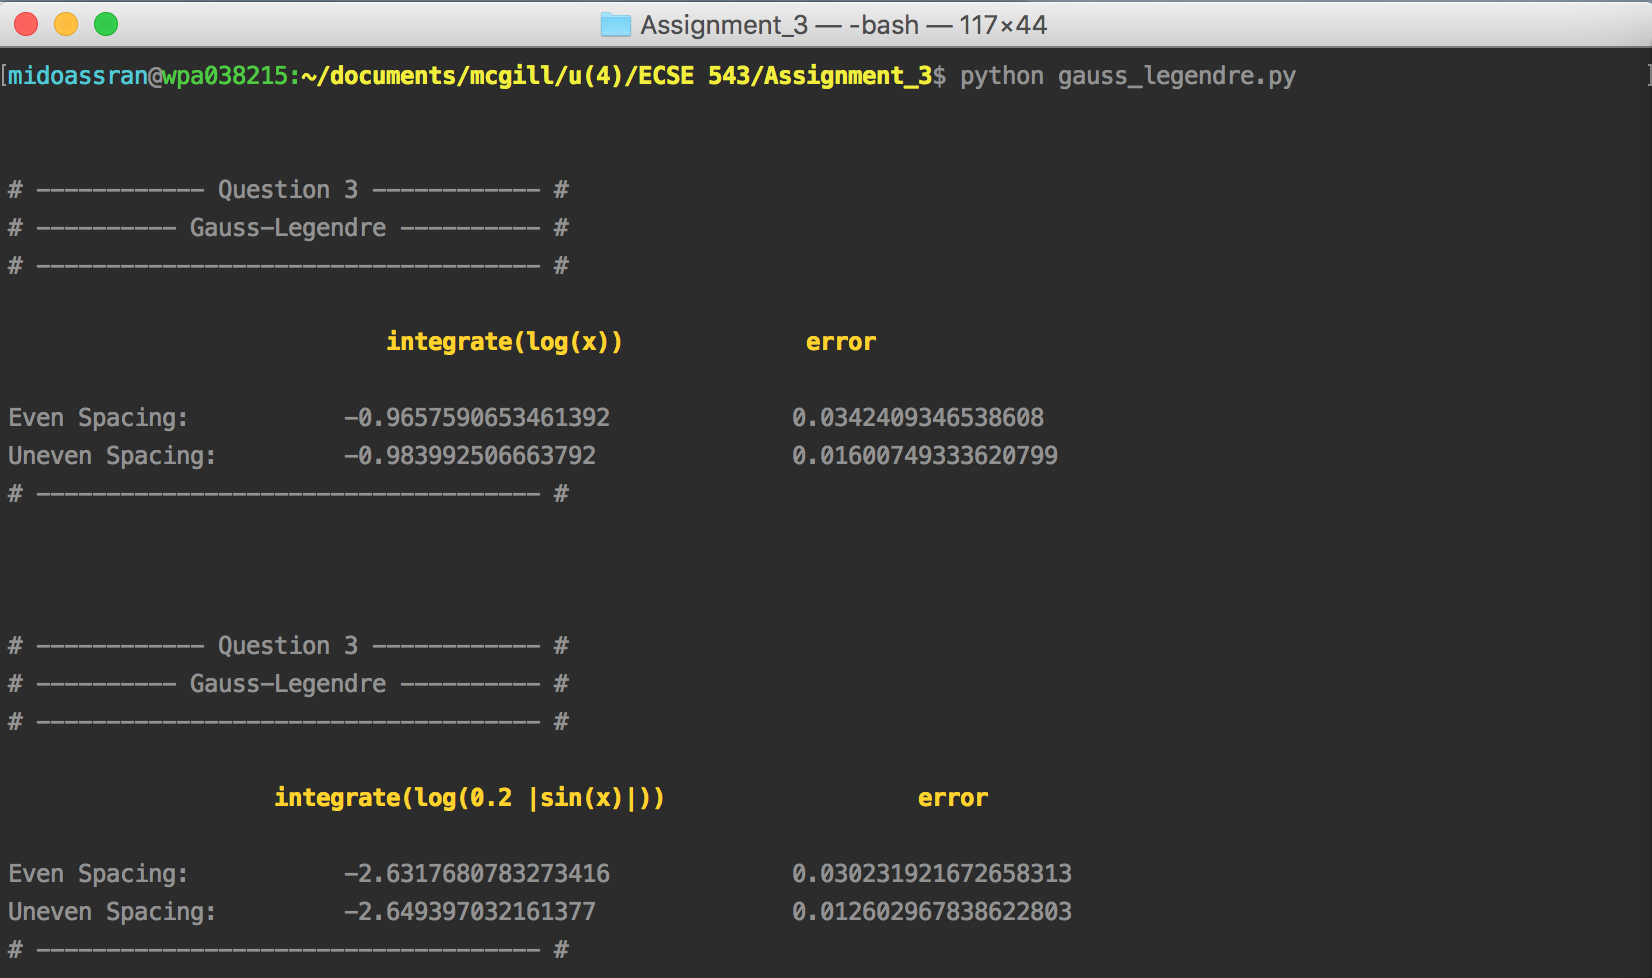
\includegraphics[width= \textwidth]{o_GL_uneven.png}\\
		\end{minipage}
		\caption{\label{fig:GL_uneven}The error in the Gauss Legendre integration of $ln(x)$ and $ln(0.2 |sin(x)|)$ over the interval $[0,1]$ for evenly spaced subintervals and unevenly spaced subintervals. The error is lower when unevenly spaced subintervals are used.}
	\end{center}
\end{figure}

\pagebreak

\begin{landscape}
    \lstinputlisting[language=Python, label=lstng:lagrange_interpolation, frame=single, caption=lagrange\_interpolation.py]{../lagrange_interpolation.py}
\end{landscape}

\begin{landscape}
    \lstinputlisting[language=Python, label=lstng:lagrange_subdomain_interpolation, frame=single, caption=lagrange\_subdomain\_interpolation.py]{../lagrange_subdomain_interpolation.py}
\end{landscape}

\begin{landscape}
    \lstinputlisting[language=Python, label=lstng:hermite_subdomain_interpolation, frame=single, caption=hermite\_subdomain\_interpolation.py]{../hermite_subdomain_interpolation.py}
\end{landscape}

\begin{landscape}
    \lstinputlisting[language=Python, label=lstng:polynomial_collective, frame=single, caption=polynomial\_collective.py]{../polynomial_collective.py}
\end{landscape}

\begin{landscape}
    \lstinputlisting[language=Python, label=lstng:polynomial, frame=single, caption=polynomial.py]{../polynomial.py}
\end{landscape}

\begin{landscape}
    \lstinputlisting[language=Python, label=lstng:newton_raphson, frame=single, caption=newton\_raphson.py]{../newton_raphson.py}
\end{landscape}

\begin{landscape}
    \lstinputlisting[language=Python, label=lstng:gauss_legendre, frame=single, caption=gauss\_legendre.py]{../gauss_legendre.py}
\end{landscape}

\begin{landscape}
    \lstinputlisting[language=Python, label=lstng:utils, frame=single, caption=utils.py]{../utils.py}
\end{landscape}

\begin{landscape}
    \lstinputlisting[language=Python, label=lstng:choleski, frame=single, caption=choleski.py]{../choleski.py}
\end{landscape}

\end{document}  















